%% bare_jrnl.tex
%% V1.4b
%% 2015/08/26
%% by Michael Shell
%% see http://www.michaelshell.org/
%% for current contact information.
%%
%% This is a skeleton file demonstrating the use of IEEEtran.cls
%% (requires IEEEtran.cls version 1.8b or later) with an IEEE
%% journal paper.
%%
%% Support sites:
%% http://www.michaelshell.org/tex/ieeetran/
%% http://www.ctan.org/pkg/ieeetran
%% and
%% http://www.ieee.org/

%%*************************************************************************
%% Legal Notice:
%% This code is offered as-is without any warranty either expressed or
%% implied; without even the implied warranty of MERCHANTABILITY or
%% FITNESS FOR A PARTICULAR PURPOSE! 
%% User assumes all risk.
%% In no event shall the IEEE or any contributor to this code be liable for
%% any damages or losses, including, but not limited to, incidental,
%% consequential, or any other damages, resulting from the use or misuse
%% of any information contained here.
%%
%% All comments are the opinions of their respective authors and are not
%% necessarily endorsed by the IEEE.
%%
%% This work is distributed under the LaTeX Project Public License (LPPL)
%% ( http://www.latex-project.org/ ) version 1.3, and may be freely used,
%% distributed and modified. A copy of the LPPL, version 1.3, is included
%% in the base LaTeX documentation of all distributions of LaTeX released
%% 2003/12/01 or later.
%% Retain all contribution notices and credits.
%% ** Modified files should be clearly indicated as such, including  **
%% ** renaming them and changing author support contact information. **
%%*************************************************************************


% *** Authors should verify (and, if needed, correct) their LaTeX system  ***
% *** with the testflow diagnostic prior to trusting their LaTeX platform ***
% *** with production work. The IEEE's font choices and paper sizes can   ***
% *** trigger bugs that do not appear when using other class files.       ***                          ***
% The testflow support page is at:
% http://www.michaelshell.org/tex/testflow/

\documentclass[conference,letterpaper,10pt,onecolumn]{IEEEtran}
\usepackage{graphicx}
\usepackage{float}
\usepackage{listings}
\floatstyle{boxed} 
\restylefloat{figure}
\usepackage[margin=0.75in]{geometry}
\usepackage{minted}
\widowpenalty10000
\clubpenalty10000




% correct bad hyphenation here
\hyphenation{op-tical net-works semi-conduc-tor}

\title{Automated Grading System
\\ \LARGE Winter Term Progress Report
\\ \Large CS 462 }

\author{Wyman, Lucy
\and Hennig, Nathan
\and Gass, Andrew}



\begin{document}
\maketitle
\begin{abstract} 
This document details the progress our group has made in the
last three months on our Automated Grading System for OSU EECS.  This includes
elements we have begun working on and details of what code has already been
written, as well as how we plan to build on these elements in the coming
months.  We also discuss problems and roadblocks we've come across, and other
interesting aspects of development thus far. It also includes plans for the
future of our project, and how we expect to complete the project.
\end{abstract}
% Turn off page numbering.
\pagenumbering{gobble}
\newpage
% Turn page numbering back on.
\pagenumbering{arabic}
\section{Project Summary}
The purpose of this project is to provide an automated grading system for EECS
classes. This will allow teachers to quickly and asynchronously provide
feedback to students, saving graders' time and improving feedback quality and
response time for students. 

Our system allows students to upload their homework to our server, which then
runs the suite of tests uploaded by the teacher on that homework.  Then, if the
teacher wants students to be able to see feedback, the system will display
which tests are or are not passing, along with hints for common errors students
might run into. Both of these features can be enabled or disabled for a
particular assignment by the teacher.

This project is particularly interesting in that we need to support tests in
multiple languages, including Python, C/C++, Ruby, and JavaScript.  Creating a
system which can successfully run tests with limited interaction from teachers,
students, or a system administrator has been the most challenging aspect of our
project.

This project also has two interfaces, a command-line interface and web
interface, both of which talk to the RESTful server to send and display data.
This server then talks to the database to create, read, update, and delete
appropriate data.

\section{Current State}

We currently have the majority of the structure for our project erected, and
are working on filling in details and trying to preempt any bugs that might
come up as we go.

We are writing the command-line interface (CLI) in Python using a powerful
module called 'cmd' that is part of the core Python library. The cmd module
provides an extremely simple framework for implementing CLIs while being
flexible enough for most purposes, including ours.

The CLI is complete except for final polishing and tweaking of output and error
reporting. All command functions have been fully implemented. All usage
information is printed dynamically from the Python dictionary we wrote that
defines all commands for the CLI. Command output is printed neatly in columns.
Using Python's basic logging module, we have implemented verbose debugging logs
to provide debugging for the implemented commands. Implemented functions are
running correctly and generating the expected output, normal and debug output
alike.

One of the more important, yet conceptually simple, pieces of our project is
the RESTful API listener server (herein referred to as the REST server)  that
will eventually live on the same server as our database. The listener server
will catch HTML packets and query the database based on those packets and
return the desired result.

The REST server is approximately ninety-five percent complete. All API calls
are detected and responded to, but a few minor, non-core features (assignment
tagging, for example) aren't working properly yet. Also, the API currently only
returns output for view commands. Other commands such as insert and update just
receive a code 200 OK response. Ideally all commands that modify the database
will receive output about those modifications as their response.

The Web UI is also being written in Python, using Django.  It is approximately
80\% completed, with most of the structural components such as forms, sitemap,
and API calls set up but not fully implements (i.e. the stub of a model exists
without it being fully or correctly defined).  The most interesting pages to
date are the registration/login page, which display an example of how a form
will look on the site and successfully communicate with the API to authenticate
users (SESSIONS still to come!), and the home page, which displays the current
courses and assignments for that individual student once they have logged in.
We ended up scrapping the idea to use CAS and have decided to use our own
methods of authentication.  The benefit to this is that we have complete
control over what information the students give us and are able to implement
authentication as we go instead of waiting until the last minute, but the
negative is that students have to individually register with our application
separately instead of being automagically added as they are with Canvas for
example.  We decided this is worth the price of admission.  

The other piece of authentication worth mentioning is that Professors must be
manually added by an approved administrator to improve security, as we could
not be certain that we would be able to create a secure way of identifying
users as teachers or students in the time allotted. This is also a hassle, but
it seemed better than the alternative of having students be able to
authenticate as professors and change their grades, which would defeat the
entire purpose of the application.

Currently, the majority of the work on the web interface will be filling in the
stubs, creating the rest of the templates and urls, ensuring that forms and
pages act as expected, and once the API is able to update the database as well
as display it ensure that that functionality works through the GUI as well.
This is entirely replicatory work, meaning that all new or unique features
have been implemented successfully and now much be repeated and tweaked to fill
out the rest of the application.  

The last major piece of our project is the testing interface. This piece caused
us some trouble at the beginning of the term, when we realized that we didn't
have a firm idea of how our client wanted testing to be performed. After
further discussion and research, we decided to implement an interface for each
language we add testing capability for. The interfaces provide output in a
standardized format, as laid out by the Test Anything Protocol (TAP). An
example of TAP output follows:

\pagebreak
\begin{lstlisting}
1..4
# Basic tests
ok 1 one equals one 
ok 2 one does not equal two 
ok 3 a true statement 
ok 4 testing works?
\end{lstlisting}

This was generated using the Python framework we implemented and a test that
uses that framework to execute a few simple tests. In addition to expecting
equality or inequality, the framework provides an �expect error� function,
which can be passed a function handle that should throw an error. The
structure for the testing functions and the Test Manager are somewhere between
alpha and beta, and can listen to the RESTful API.We still need to expand the
testing.

\section{Problems}

There were a number of problems with the CLI. The main problem was that we
failed to consider the need to specifically design the command structure for
the CLI, and failed to budget time to do so. The CLI design was completed
around the end of week 3, although we are still fixing minor flaws as we find
them, and the command structure is not fully consistent in all places (in other
words, some commands use one argument pattern while similar commands use a
different argument pattern). 

Ideally, we will solve this problem by going back through the design and
reworking it entirely. We may do that later depending on how much time we have
to polish the interface. 

The second problem with CLI was that after implementing about half the commands
we noticed that code reuse was a problem. Many of the commands use code that
similar to other commands, but not quite similar enough to be easily moved into
a helper function.

We solved this problem by going through the design and making small changes
that reduced syntactical variations between commands. Those changes allowed us
to create a single set of execution functions that can process all commands
based on their design in the Python command dictionary. This modular approach
eliminated code reuse and makes it so that any changes to the command structure
of the CLI will be easy to implement.  

There have also been some unforeseen troubles with the Web UI. First is the URL
and authentication issue.  A few months  ago we contacted EECS to ask about
getting a subdomain for our application, and they notified us that even with
the help of our mentor this wouldn't be possible until much closer to Expo.
Because of this, we couldn't authorize the application with the Central
Authentication Services, which we were planning on using for authentication.
So, we decided to set up our own login system, initially thinking it would be
temporary but then deciding that it was necessary to properly authenticate our
users and would be production quality.  

Then there were unexpected difficulties with setting up a basic login system to
use in place of CAS for development.  For a while I had a difficult time
getting login to actually talk to my local database, but since that wasn't what
we were planning on doing in production (the UI will talk to the database
through an API, and it won't necessarily be local), I scrapped that and have
decided to authenticate using the methods we'll be using in production, which
do actually work.  In retrospect this was a pretty minor and inconsequential
roadblock, but at the time it was very frustrating.

As stated above in the status section, the testing section of our project gave
us some issues after we realized that we hadn't adequately define requirements
for that section during the design phase. We were able to solve this problem by
researching various testing methods and looking at sites like CodeWars.com that
focus on code testing. We eventually settled on a framework based on the
CodeWars design for katas that generates Test Anything Protocol (TAP) output.

On the implementation side of the manager and testers, we used a
multiprocessing approach to handle the expected load. An arbitrary number of
testers may be launched with the manager, and which uses two threads to ensure
that dispensing tests to testers never blocks responses to requests from either
of the UIs. This should ensure expandability, stability, and responsiveness
under load.

\section{Plans}

The CLI is essentially complete at this point, so we plan to spend time trying
different ways of displaying output and fixing any bugs we discover as we
continue testing.

For the REST API, we plan to continue testing and debugging it, as well as
implementing the tags feature. We also want to finish implementing
authentication through the database.


For the Web UI, all that is left to do is fill in the rest of the
application, replicating and tweaking functionality we already have (ie.
creating the rest of the forms and web pages, filling out the sitemap
structure, and making all the correct API calls).  We don't foresee any major
roadblocks with this as the actual functionality has already been tested and is
working, and now we are just filling in the stubs for the rest of the
application.

\pagebreak
The implementation of the testing framework should be fairly straightforward.
We don't expect the initial issues to cause problems with hitting the beta
release since we're now following a well-conceived design, and most of the work
going forward will be linking with the database, as well as writing interfaces
with more languages and deciding on the extent we plan to support
multi-language tests.

\section{Code Snippets}
\subsection{Web Interface (GUI)}
Listing 1 is an example of querying the API for data to be displayed on a 
web page, parsing the data, and then rendering the page. This is part 
of the core functionality of the web interface part of the system, is 
just talking to the API, parsing that input/output, and then displaying it.
\begin{listing}[H]
    \begin{minted}[linenos]{python}
def index(request):
	api_ip = settings.API_IP
	user_data = {'student':['hennign']}
	userobj = requests.get(api_ip+'student/view', json=user_data)
	user = userobj.json()
	for i in range(len(user)):
		user[i]['type'] = 'student'
	courses = []
	for course in user:
		course_data = {'course-id':[course['course_id']]}
		cobj = requests.get(api_ip+'course/view', json=course_data)
		c = cobj.json()
		aobj = requests.get(api_ip+'assignment/view')
		c[0]['assignments'] = aobj.json()
		courses.append(c[0])
	return render_to_response('index.html', {'n':datetime.datetime.now(), 
                              'user':user[0], 'courses':courses})
    \end{minted}
    \caption{View function for the index page}
\end{listing}

The other core functionality is getting data from users to put in the database,
which is done through forms like the one created in Listing 2.

\begin{listing}[H]
    \begin{minted}[linenos]{python} 
class NewUser(forms.Form):
	first_name = forms.CharField(label='First Name', required=True)
	last_name = forms.CharField(label='Last Name', required=True)
	##TODO ask to re-enter onid
	onid = forms.CharField(label='ONID ID Number', required=True)
	usertype = forms.ChoiceField(choices=TYPES,
			required=True, label='Are you a Professor, TA, or student?')
	password = forms.CharField(label='Password',
                               required=True,
                               widget=forms.PasswordInput)
	password2 = forms.CharField(label='Re-enter Password',
                                required=True,
                                widget=forms.PasswordInput)
    \end{minted}
    \caption{Example of a form}
\end{listing}

\subsection{Command Line Interface}
The CLI is implemented using the module 'cmd', one of the core Python modules.
Due to the robustness of said module, most of the CLI code is very
straightforward. Here are a few samples of the code that weren't
straightforward.

\begin{listing}[H]
    \begin{minted}[linenos]{python}
def print_response(self, command, subcommand, json):
	data = json

	cols = [x for x in sql_dict.sql[command][subcommand]['view_order'] 
			if x in data[0]]
	col_widths = [max([len(str(row[key])) for row in data] + \
			[len(str(key))]) + 4 for key in cols]


	sort_order = [x 
			for x in sql_dict.sql[command][subcommand]['sort_order'] 
			if x in data[0]]

	print("|".join(str(val).center(col_widths[pos]) 
			for pos,val in enumerate(cols)))
	print("|".join(str("="*(col_widths[pos]-2)).center(col_widths[pos]) 
			for pos,val in enumerate(cols)))

	data.sort(key = lambda x: [x[key] for key in sort_order])

	for row in data:
		print("|".join(str(row[val]).center(col_widths[pos]) 
				for pos,val in enumerate(cols)))
    \end{minted}
    \caption{CLI code responsible for printing the view commands results returned from the REST API}
\end{listing}

Listing 3 shows the CLI helper function print\_response. This function takes a
command, subcommand, and the json from a HTTP response and processes it into
nice looking columns as seen in Figure 1. First the view and sort orders are
checked against the data to see which columns are present in the data. Then a
list of column widths is built using the maximum length of the values for each
key or length of the key name, whichever is longer. After printing the column
headers, the json data is sorted by the sort order keys and then each row is
printed.

This piece of code is important, because this view output is what users will
see most frequently. The output needs to be well formated, both to impress the
users and to improve the usability of the CLI.

\begin{figure}[H]
\centering
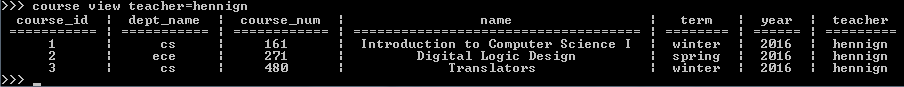
\includegraphics[width=0.8\textwidth]{senior-project-course-view-output}
\caption{Screenshot of CLI output from course view command showing column formatted data.}
\end{figure}

\begin{listing}[H]
    \begin{minted}[linenos]{python}
undoc_header = None
def print_topics(self, header, cmds, cmdlen, maxcol):
	if header is not None:
		cmd.Cmd.print_topics(self, header, cmds, cmdlen, maxcol)
    \end{minted}
    \caption{CLI code responsible for hiding undocumented commands from help}
\end{listing}

By default, when the \texttt{help} command is run, undocumented commands are
prefaced with the string in undoc\_header and listed out. This behavior is
undesirable, since the only undocumented commands are things like \texttt{EOF}
and exit, where having help files would be awkward and confusing. Listing 4
demonstrates how we fix this issue.

The function print\_topics is a built-in function of the cmd module from which
the AutoShell class inherits and is used to print command lists for the various
help categories. Here we override the function with our own copy which checks
to see is the \texttt{header} is not equal to \texttt{None}. If this evaluates
as true, then we call the original version of the function. If it is false,
then we do nothing. This allows us to get the desired behavior without
completely reimplementing the inherited function.

\subsection{REST API}

\begin{listing}[H]
    \begin{minted}[linenos]{python}
for table in tables:
	query = """SELECT tc.constraint_name, tc.table_name, kcu.column_name,
			ccu.table_name AS foreign_table_name,
			ccu.column_name AS foreign_column_name
		FROM information_schema.table_constraints AS tc
		JOIN information_schema.key_column_usage AS kcu
		ON tc.constraint_name = kcu.constraint_name
		JOIN information_schema.constraint_column_usage AS ccu
		ON ccu.constraint_name = tc.constraint_name
		WHERE constraint_type = 'FOREIGN KEY' 
              AND tc.table_name = %(tablename)s"""
	cur.execute(query, table)
	for row in cur.fetchall():
		constraint, table, column, foreign_table, foreign_column = row
		edges.append([row['table_name'], row['foreign_table_name'],
			row['column_name'], row['foreign_column_name']])
    \end{minted}
    \caption{Generating a list of edges for tables in a PostgreSQL database from the information schema tables}
\end{listing}

Some of the most interesting code in the REST server is related to the way the
API builds queries for the view commands. At first we considered writing each
query by hand, but after careful consideration we decided that it would
ultimately save time if the view queries were generated automatically.
Relational databases can be thought of as graphs where each table is a node
with edges created by foreign key constraints. PostgreSQL stores this data
automatically in the information\_schema tables. This data can later be
extracted (see Listing 5) and used to represent a set of edges between tables.

The code in Listing 5 is important because it is the first step in building a
graph that can be used to automatically generate joins for any given set of
tables in the graph. Automatically generating joins this way allows easy
modification of the view commands, thereby increasing the maintainability of
the REST server.

\begin{listing}[H]
    \begin{minted}[linenos]{python}
elif 'multipart/form-data' in self.headers['Content-Type']:
	form = cgi.FieldStorage(
		fp=self.rfile,
		headers=self.headers,
		environ={'REQUEST_METHOD':'POST',
		})

	data = {}
	for key in form.keys():
		if key not in ['file', 'filepath']:
			variable = str(key)
			value = str(form.getvalue(variable))
			self.logger.debug("value: {0}".format(value))

			try:
				data[variable] = ast.literal_eval(value)
			except:
				data[variable] = [str(value)]

			if type(data[variable]) != type([]):
				data[variable] = [str(value)]
	fileitem = form['file']

	# Test if the file was uploaded
	if fileitem.filename:
		fn = os.path.basename(fileitem.filename)
		open(os.path.normpath(sql['basedir'] + fn),
             'wb').write(fileitem.file.read())
    \end{minted}
    \caption{Processing a multipart/form-data HTTP request using cgi.FieldStorage and saving a file to disk}
\end{listing}

While the data from Content-Type \texttt{application/json} can easily be parsed,
\texttt{multipart/form-data} is more complex. Luckily we determined that the cgi
module was capable of automatically processing such a request, as shown in
Listing 6. Once the data has been read into a FieldStorage object, getting the
various variables was as simple as looping through the keys and pulling the
values out. Listing 6 also shows how we saved the file data to disk for later
use.

One of the more important tasks of the REST server is processing calls that
include file data. One of the core requirements of our project is that users
are able to submit files that are then tested. Without the code in Listing 6,
any attempt to submit a file would fail.
\subsection{Testing Framework}
\begin{listing}[H]
    \begin{minted}[linenos]{python}
class dispenserThread (threading.Thread):
def __init__(self):
	threading.Thread.__init__(self)
def run(self):
	print('Dispenser thread running')
	while True:
		qlock.acquire()
		while True:
			l = len(testQ)
			if(l > 0):
				break
			qlock.wait()
	sub_ID = testQ.popleft()
	qlock.release()
	tester = -1
	tlock.acquire()
	while True:
		try:
			tester = testers.index(0)
		except Exception:
			pass
		if(tester > -1):
			break
		tlock.wait()
	testers[tester] = int(sub_ID)
	tlock.release()
	s.connect('\0recvPort' + str(tester))
	msg = '{"sub_ID":' + str(sub_ID) + '}'
	s.send(msg.encode())
	s.close()
    \end{minted}
    \caption{Dispenser thread for my herald process. Wait, send.}
\end{listing}
The dispenser thread (Listing 7) works with the tester processes, checking for a pending
test first, then checking for processes without a current test. Both are
performed with Python condition blocking. In addition, upon assigning a test to
a tester, the submission ID is stored in the tester's index.  The main thread's
'matched' code:

\begin{listing}[H]
    \begin{minted}[linenos]{python}
while running:
	readlist,writelist,exceptlist = select.select([c,k,r],[],[])
	for avail in readlist:
		if avail is c:
			h = c.accept()[0]
			msg = h.recv(256)
			h.close()
			dmsg = msg.decode()
			sub_ID = json.loads(dmsg)["sub_ID"]

			#TESTING LINE
			sub_ID = 83

			qlock.acquire()
			testQ.append(sub_ID)
			qlock.notify()
			qlock.release()
		elif avail is k:
			print("Herald recieved kill signal")
			remv = k.accept()[0]
			for j in range(int(sys.argv[1])):
			o = socket.socket(socket.AF_UNIX,socket.SOCK_STREAM);
			o.connect('\0killPort' + str(j))
			o.send('{"state":"die"}'.encode())
			o.close()
			k.close()
			exit()
		elif avail is r:
			rec = r.accept()[0]
			msg = rec.recv(256)
			dmsg = msg.decode()
			sub_ID = json.loads(dmsg)["sub_ID"]
			tlock.acquire()
			try:
				idx = testers.index(int(sub_ID))
				testers[idx] = 0
				print('Submission evaluated.')
			except ValueError:
				print("Error: a test was reported completed, but no record of it being started.")
			tlock.notify()
			tlock.release()
			rec.close
    \end{minted}
    \caption{Main loop of my herald (manage) process.}
\end{listing}

The select tree (Listing 8) allows non-blocking port listening. If a new test is registered
on the socket bound to 'c', then it is registered in a FIFO queue, and the
thread condition is notified in case the dispenser was waiting on that. The 'r'
socket will will hear back from the testers and mark the tester process done,
then notify of the freed process. The 'k' socket is a cleanup socket that
closes out all the tester processes. Finally, the testing framework for Python
is on the following page:

\begin{listing}[H]
    \begin{minted}[linenos]{python}
import operator

class test_suite:
	def __init__(self):
		self.testcount = 0
		self.testsremain = 0

	#Helper functions
	def ok(self,message):
		self.testcount += 1
		self.testsremain -= 1
		if(self.testsremain < 0): print(
            '# Exceeded declared test count for this "describe"!')
		print('ok ' + str(self.testcount) + ' ' + message)
	def notok(self,message):
		self.testcount += 1
		self.testsremain -= 1
		if(self.testsremain < 0): print(
            '# Exceeded declared test count for this "describe"!')
		print('not ok ' + str(self.testcount) + ' ' + message)

	#Testing functions
	def assert_equals(self,actual,expected,message):
		if(operator.eq(actual,expected)):
			self.ok(message)
		else:
			self.notok(message)
	def assert_not_equals(self,actual,unexpected,message):
		if(operator.ne(actual,unexpected)):
			self.ok(message)
		else:
			self.notok(message)
	def expect_error(self,message,thunk):
		try:
			thunk()
			self.notok(message)
		except:
			self.ok(message)
	def expect(self,passed,message):
		if(passed):
			self.ok(message)
		else:
			self.notok(message)

	#Grouping functions
	def describe(self,message,tests):
		print(str(self.testcount + 1) + '..' + str(self.testcount + tests))
		print('# ' + message)
		self.testsremain = tests
	def it(self,message):
		print('# ' + message)
    \end{minted}
    \caption{Python testing framework. Used to generate TAP output from a test suite.}
\end{listing}

Here in the test\_suite (Listing 8) are the implementations for the testing functions. 
They reference back toprint functions for their results, and the comparison relies 
on Python's \texttt{operator} library, a functionality we may need to implement 
separately in other languages.

\section{Screenshots}
Below are screenshots of relevant aspects of our system which are particularly
visual, or can be clarified visually.
\subsection{Web Interface (GUI)}
The index page, being the home of the site and the first page is most people 
see, so it needs to be done right!  Students should ideally be able to access
most, if not all, other parts of the website from this page. For that reason
we included a list of courses and their relevant assignments, and will add
links to upload a submission for that assignment if it is not past due.
\begin{figure}[H]
	\centering
	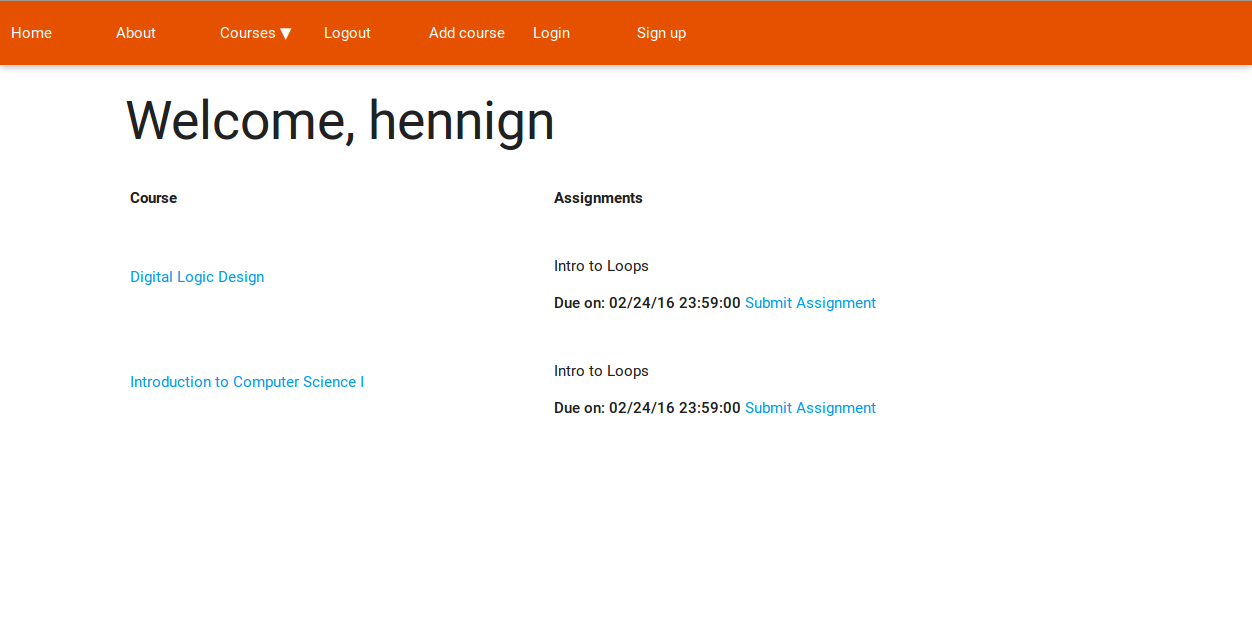
\includegraphics[width=0.8\textwidth]{index-page}
	\caption{Demo of the home page for the website}
\end{figure}

As stated previously, we also require the students register with our application
individually, so needed a registration page as well.

\begin{figure}[h]
\centering
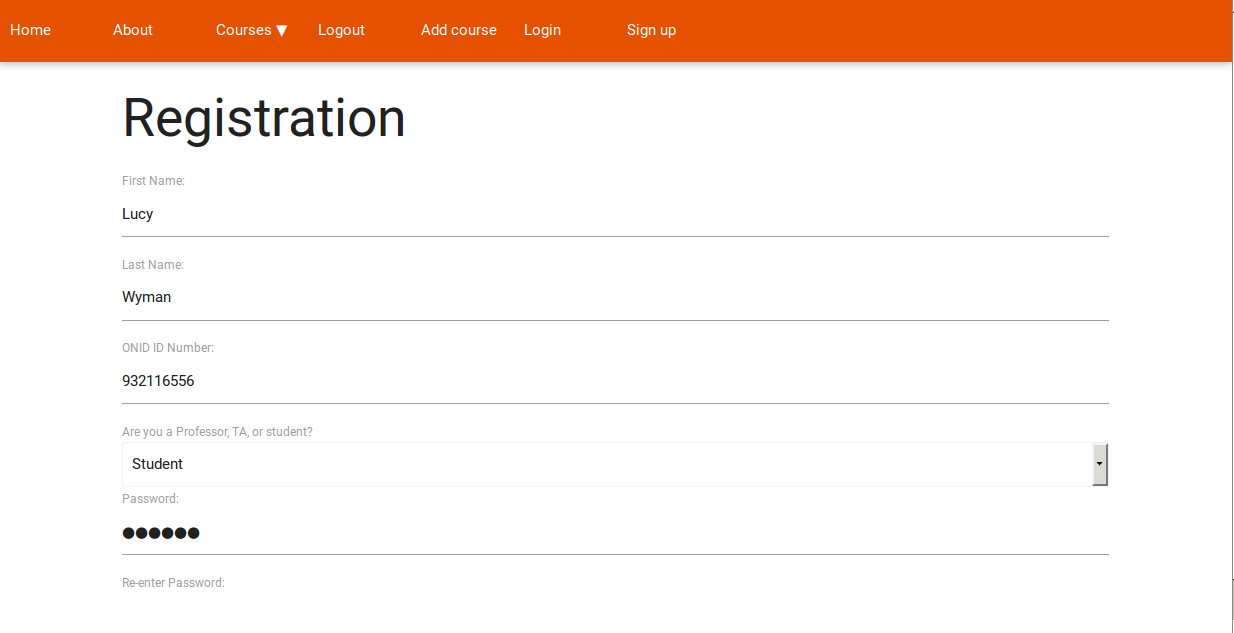
\includegraphics[width=0.8\textwidth]{register}
\caption{Demo of the Registration page, where students must create an account}
\end{figure}

\pagebreak
\subsection{Command Line Interface}
The nature of a command line interface is such that it doesn't really lend
itself interesting screenshots, but in order to demonstrate how the CLI looks,
we've included a few here.

\begin{figure}[h]
\centering
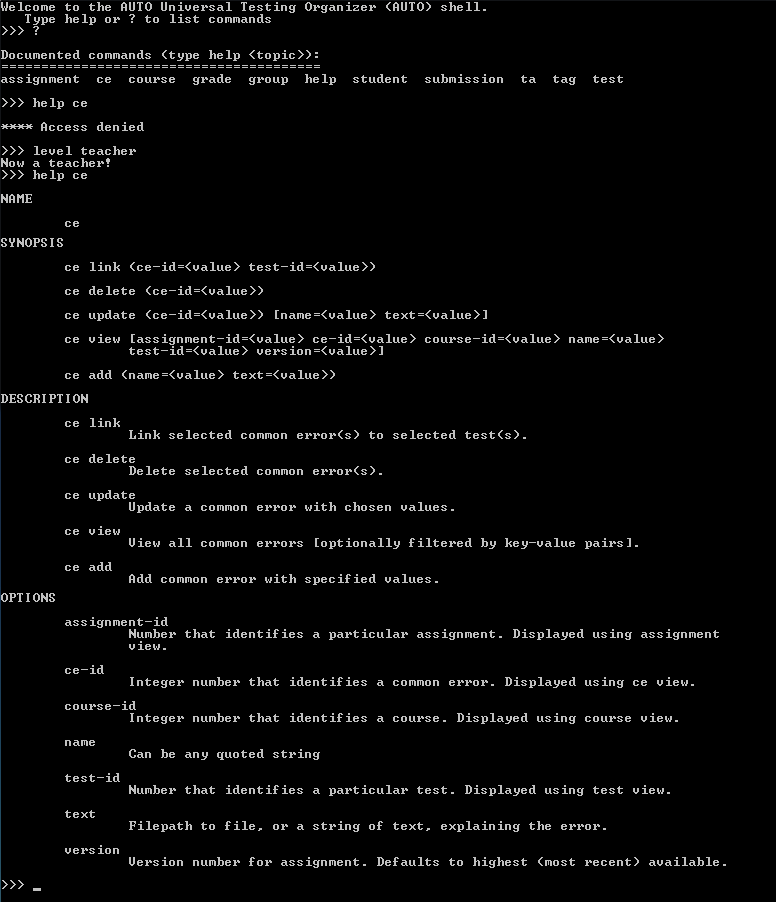
\includegraphics[width=0.8\textwidth]{senior-project-screenshot-CLI-help-ce}
\caption{Demonstrating opening message of the CLI and the output of 'help ce'.}
\end{figure}

Figure 4 demonstrates a few interesting aspects of the CLI. The first is the
welcome message, which welcomes the user and explains how to use the help
command to see other commands. Next we use the 'level' command to change access
levels while also using 'help ce' command to show how a help file looks
different depending on your access level.

\begin{figure}[h]
\centering
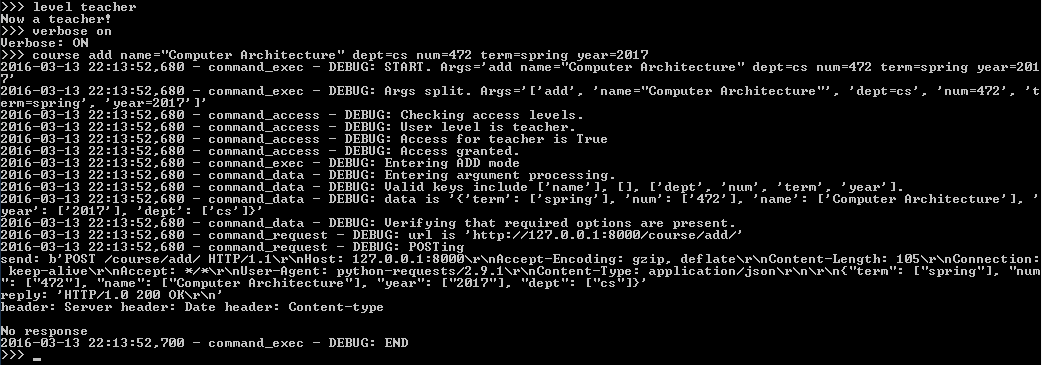
\includegraphics[width=0.8\textwidth]{senior-project-screenshot-CLI-verbose-add-course}
\caption{Demonstration of the course command with debugging active.}
\end{figure}

Figure 5 shows a test run of the \texttt{course} command with verbose on.
Verbose is a testing command that will most likely either be removed from the
released version or restricted to teachers. The CLI has been written using
Python's logging module to insert debug messages. The verbose command allows
the user to change the logging level from warning to debug and back.

As can be seen from the debug messages above, the attempt to run the
\texttt{course} command worked beautifully. All the arguments were parsed
correctly and the API call was made correctly. Unfortunately, the REST server
doesn't implement the course command yet, so it returned a \texttt{501
Unsupported} method' error as its response.


\pagebreak
\section{Conclusion}
We are pleased to report that our  beta version is essentially complete, just
as we planned. All that is left for the core of our project is to properly
integrate authentication. Right now there are a few places that should be
checking for access rights that aren't, but we expect implementation to consist
of little more than a few short functions. Otherwise we expect to be focused
on polishing code and adding a few bonus features as schedules permit.
\end{document}
